% Created 2019-03-26 Tue 22:29
% Intended LaTeX compiler: pdflatex
\documentclass[12pt, aspectratio=1610]{beamer}

\usepackage{appendixnumberbeamer}
\usepackage[utf8]{inputenc}
\usepackage{ngerman}
\definecolor{sbase03}{HTML}{002B36}
\definecolor{sbase02}{HTML}{073642}
\definecolor{sbase01}{HTML}{586E75}
\definecolor{sbase00}{HTML}{657B83}
\definecolor{sbase0}{HTML}{839496}
\definecolor{sbase1}{HTML}{93A1A1}
\definecolor{sbase2}{HTML}{EEE8D5}
\definecolor{sbase3}{HTML}{FDF6E3}
\definecolor{red}{HTML}{DC322F}
\definecolor{pink}{HTML}{D33682}
\definecolor{purple}{HTML}{6C71C4}
\definecolor{blue}{HTML}{268BD2}
\definecolor{brown}{HTML}{795548}
\definecolor{cyan}{HTML}{2AA198}
\definecolor{darkgray}{HTML}{616161}
\definecolor{gray}{HTML}{9E9E9E}
\definecolor{lightgray}{HTML}{E0E0E0}
\definecolor{lime}{HTML}{CDDC39}
\definecolor{olive}{HTML}{827717}
\definecolor{orange}{HTML}{CB4B16}
\definecolor{teal}{HTML}{009688}
\definecolor{yellow}{HTML}{B58900}
\definecolor{green}{HTML}{859900}
\usepackage{listings}
\usepackage{color}
\usepackage{sourcecodepro}
\lstset{
  breaklines,
  literate={ö}{{\"o}}1
           {ä}{{\"a}}1
           {ü}{{\"u}}1,
  captionpos=b,                    % sets the caption-position to bottom
  sensitive=true,
  xleftmargin=\parindent,
  escapeinside={\%*}{*)},          % if you want to add LaTeX within your code
  basicstyle=\color{sbase00}\ttfamily,
  keywordstyle=\color{cyan},
  commentstyle=\color{sbase1},
  stringstyle=\color{blue},
  numberstyle=\color{purple},
  identifierstyle=\color{sbase00},
  showstringspaces=false,          % Removes the strange symboles where spaces are
}

\usepackage[most]{tcolorbox}
\newtcblisting{sexylisting}[2][]{
  sharp corners,
  fonttitle=\bfseries,
  colframe=gray,
  listing only,
  listing options={
    basicstyle=\color{sbase00}\ttfamily,
    keywordstyle=\color{cyan},
    commentstyle=\color{sbase1},
    stringstyle=\color{blue},
    numberstyle=\color{purple},
    identifierstyle=\color{sbase00},
    language=C,
  },
  title=\thetcbcounter #2, #1
}
\useoutertheme{sidebar}
\usetheme{metropolis}
\author{Andreas Zweili}
\date{\today}
\title{Präsentation Diplomarbeit}
\hypersetup{
 pdfauthor={Andreas Zweili},
 pdftitle={Präsentation Diplomarbeit},
 pdfkeywords={},
 pdfsubject={},
 pdfcreator={Emacs 26.1 (Org mode 9.2.2)},
 pdflang={Germanb}}
\begin{document}

\maketitle\newpage
\begin{frame}{Inhalt}
\tableofcontents
\end{frame}


\section{Einführung}
\label{sec:orge023b06}
\begin{frame}[label={sec:org9f49b5e}]{Einführung}
\begin{itemize}
\item <2-> Grafische Oberfläche für das \newline Kommandozeilen Programm "`BorgBackup"'
\item <3-> Evaluation der Technologien
\item <4-> Programmieren der Basis-Funktionen
\end{itemize}
\end{frame}

\begin{frame}[label={sec:org25c7176}]{Einführung}
\begin{columns}
\begin{column}{0.5\columnwidth}
\alert{Inspiration}
\begin{itemize}
\item <2-> Fehlende Backups im Umfeld
\item <3-> Fehlendes Know-How im Umfeld
\item <4-> Software "`Back in Time"'
\end{itemize}
\end{column}

\begin{column}{0.5\columnwidth}
\begin{center}
\includegraphics[width=.9\linewidth]{pictures/inspiration.png}
\end{center}
\end{column}
\end{columns}
\end{frame}

\begin{frame}[label={sec:org4ab726b}]{Einführung}
\begin{columns}
\begin{column}{0.5\columnwidth}
\alert{Wieso BorgBackup?}
\begin{itemize}
\item <3-> Open Source Software
\item <4-> War cross-plattform fähig
\item <5-> Blockbasierte Deduplikation
\end{itemize}
\end{column}

\begin{column}{0.5\columnwidth}
\begin{center}
\includegraphics[width=.9\linewidth]{pictures/borg.jpeg}
\end{center}
\end{column}
\end{columns}
\end{frame}

\begin{frame}[label={sec:orgc1dff6b}]{Einführung}
\alert{Blockbasierte Deduplikation}

\begin{center}
\includegraphics[width=.9\linewidth]{pictures/deduplication.png}
\end{center}
\end{frame}


\section{Projekt Management}
\label{sec:org7c0fc40}
\begin{frame}[label={sec:org26940da}]{Projekt Mangement}
\begin{columns}
\begin{column}{0.5\columnwidth}
\alert{Wasserfallmodell}
\begin{itemize}
\item <2-> Funktioniert gut für Einzelpersonen
\item <3-> Phasenbasiertes Modell
\end{itemize}
\end{column}

\begin{column}{0.5\columnwidth}
\begin{center}
\includegraphics[width=.8\linewidth]{pictures/waterfall_stairs.jpg}
\end{center}
\end{column}
\end{columns}
\end{frame}

\begin{frame}[label={sec:org31b6f31}]{Projekt Management}
\begin{columns}
\begin{column}{0.45\columnwidth}
\alert{Ist-Risiko}
\begin{itemize}
\item <2-> Ungewohnte Nutzung einer Kommandozeilen Applikation
\item <3-> Backups ohne Verschlüsselung
\item <4-> Falscher Speicherort
\item <5-> Versehentliche Löschung
\item <6-> User vergisst Backups zu machen
\end{itemize}
\end{column}

\begin{column}{0.45\columnwidth}
\begin{center}
\includegraphics<2>[width=\linewidth]{pictures/istrisiko1.pdf}%
\includegraphics<3>[width=\linewidth]{pictures/istrisiko2.pdf}%
\includegraphics<4>[width=\linewidth]{pictures/istrisiko3.pdf}%
\includegraphics<5>[width=\linewidth]{pictures/istrisiko4.pdf}%
\includegraphics<6>[width=\linewidth]{pictures/istrisiko.pdf}%
\end{center}
\end{column}
\end{columns}
\end{frame}

\begin{frame}[label={sec:org3a5c2b2}]{Projekt Mangement}
\begin{columns}
\begin{column}{0.45\columnwidth}
\alert{Ist-Risiko}
\begin{center}
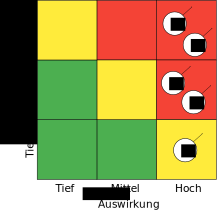
\includegraphics[width=\linewidth]{pictures/istrisiko.pdf}%
\end{center}
\end{column}

\begin{column}{0.45\columnwidth}
\onslide<2->\alert{Soll-Risiko}
\begin{center}
\includegraphics<2->[width=\linewidth]{pictures/sollrisiko.pdf}%
\end{center}
\end{column}
\end{columns}
\end{frame}

\begin{frame}[label={sec:org5c7b81d}]{Projekt Mangement}
\begin{block}{Controlling}
\end{block}
\end{frame}

\section{Varianten}
\label{sec:org15ff9ea}
\begin{frame}[label={sec:org15f8ca7}]{Varianten}
\alert{Kriterien}
\begin{itemize}
\item <2-> Cross-plattform kompatibel
\item <3-> Freie Software
\item <4-> Vorkenntnisse
\item <5-> Integriert sich gut ins System
\item <6-> Ohne spezielle Tools nutzbar
\end{itemize}
\end{frame}

\begin{frame}[label={sec:org5d04a57}]{Varianten}
\begin{columns}
\begin{column}{0.3\columnwidth}
\alert{Backend}
\begin{itemize}
\item <2-> C\#
\item <3-> Python
\item <4-> C++
\end{itemize}
\end{column}

\begin{column}{0.5\columnwidth}
\begin{center}
\includegraphics<2>[width=\linewidth]{pictures/backend1.png}%
\includegraphics<3>[width=\linewidth]{pictures/backend2.png}%
\includegraphics<4>[width=\linewidth]{pictures/backend3.png}%
\end{center}
\end{column}
\end{columns}
\end{frame}

\begin{frame}[label={sec:org260fa3e}]{Varianten}
\alert{Frontend}
\end{frame}

\begin{frame}[label={sec:org0e7c972}]{Varianten}
\begin{columns}
\begin{column}{0.3\columnwidth}
\alert{Frontend}
\begin{itemize}
\item <2-> Qt
\item <3-> Gtk
\item <4-> Electron
\end{itemize}
\end{column}

\begin{column}{0.5\columnwidth}
\begin{center}
\includegraphics<2>[width=.9\linewidth]{pictures/frontend1.png}%
\includegraphics<3>[width=.9\linewidth]{pictures/frontend2.png}%
\includegraphics<4>[width=.9\linewidth]{pictures/frontend3.png}%
\end{center}
\end{column}
\end{columns}
\end{frame}

\begin{frame}[label={sec:org14d576a}]{Varianten}
\alert{Resultat}

\begin{center}
\includegraphics[height=.5\textheight]{pictures/pyqt.png}
\end{center}
\end{frame}

\section{Umsetzung}
\label{sec:orga98862e}
\begin{frame}[label={sec:org96597b8}]{Umsetzung}
\begin{columns}
\begin{column}{0.3\columnwidth}
\alert{Werkzeuge}

\begin{itemize}
\item <2-> Gnome Planner
\item <3-> Emacs
\item <4-> Git
\item <5-> Qt-Designer
\item <6-> Inkscape
\item <7-> Draw.io
\item <8-> Virtualbox
\end{itemize}
\end{column}

\begin{column}{0.5\columnwidth}
\begin{center}
\includegraphics<2>[width=.9\linewidth]{pictures/tools1.png}%
\includegraphics<3>[width=.9\linewidth]{pictures/tools2.png}%
\includegraphics<4>[width=.9\linewidth]{pictures/tools3.png}%
\includegraphics<5>[width=.9\linewidth]{pictures/tools3.png}%
\includegraphics<6>[width=.9\linewidth]{pictures/tools5.png}%
\includegraphics<7>[width=.9\linewidth]{pictures/tools6.png}%
\includegraphics<8>[width=.9\linewidth]{pictures/tools7.png}%
\end{center}
\end{column}
\end{columns}
\end{frame}

\begin{frame}[label={sec:org999a1cb}]{Umsetzung}
\alert{Finales Produkt}

\begin{center}
\includegraphics[height=.8\textheight]{pictures/borgqt1.png}%
\end{center}
\end{frame}

\begin{frame}[label={sec:orgee133bf}]{Umsetzung}
\alert{Finales Produkt}

\begin{center}
\frame{\includegraphics[width=\textwidth]{pictures/borgqt5.png}}%
\end{center}
\end{frame}

\begin{frame}[label={sec:org60e3ecf}]{Umsetzung}
\begin{center}
\begin{tabular}{ll}
\textbf{Speicherverbrauch} & \\
\hline
Reale Grösse & 13.41 TB\\
Deduplizierte Grösse & 556.67 GB\\
\end{tabular}

\end{center}

\begin{center}
24x weniger Speicherverbrauch
\end{center}
\end{frame}

\begin{frame}[label={sec:orgc5d4229}]{Umsetzung}
\begin{columns}
\begin{column}{0.45\columnwidth}
\alert{Soll-Risiko}
\begin{center}
\includegraphics[width=\linewidth]{pictures/sollrisiko_grey.pdf}%
\end{center}
\end{column}

\begin{column}{0.45\columnwidth}
\onslide<2->\alert{Neues Ist-Risiko}
\begin{center}
\includegraphics<2->[width=\linewidth]{pictures/ist_risiko_neu.pdf}%
\end{center}
\end{column}
\end{columns}
\end{frame}

\section{Abschluss}
\label{sec:org17a94ab}
\begin{frame}[label={sec:org1bf9035}]{Abschluss}
\alert{Fazit}
\begin{itemize}
\item <2-> Die Arbeit war sehr interessant und zeitintensiv
\item <3-> Ganttcharts können sehr hilfreich sein um den Fokus zu halten
\item <4-> Unittests sind ein Must-have für Entwickler sind jedoch auch zeitintensiv
\item <5-> Mehr Erfahrung im Bereich "`Test-Driven-Developement"' sammeln
\end{itemize}
\end{frame}

\begin{frame}[label={sec:orgccda786}]{}
\alert{\huge{Fragen?}}
\end{frame}
\begin{frame}[label={sec:org5fbcdb2}]{}
\alert{\huge{Vielen Dank für die Aufmerksamkeit!}}
\end{frame}
\end{document}